\chapter{Principal Component Analysis}
\section{Introduction}
In Principal Component Analysis the goal is to represent $N$-dimensional data using less then N numbers. This is done by finding $M$ orthogonal directions in which the data have the most variance and ignore the directions in where the data do not variance much. These $M$ principal directions form a lower-dimensional subspace and a $N$-dimensional data point can be represented by its projections onto these $M$ directions in the lower dimension subspace. The information about where the data is located in the remaining $N-M$ orthogonal directions are therefore lost. Since these do not have much variance, only a little information is lost.

\section{Percent Variance Explained by $M$ Components}
\begin{figure}[hbtp]
\centering
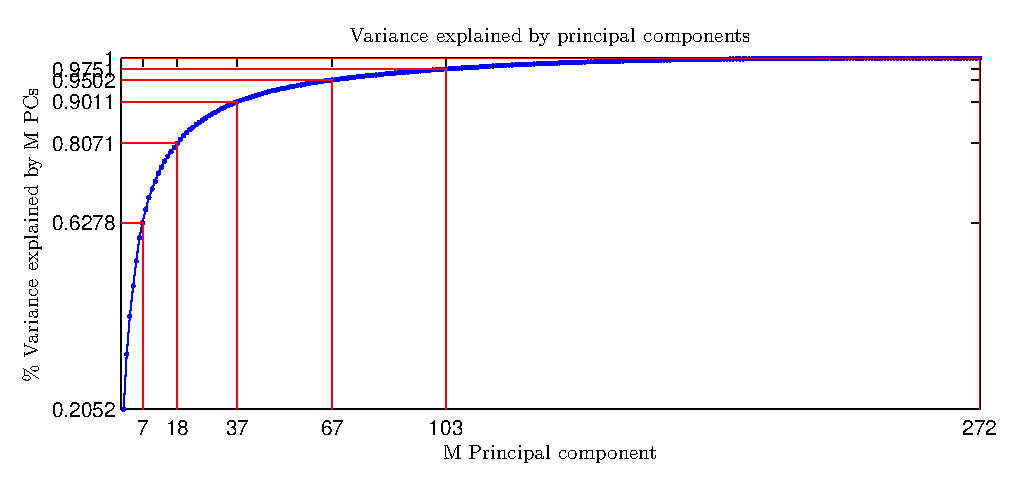
\includegraphics[width=\linewidth]{var_explained}
\caption{The variance explained by $M$ Components.\label{fig:pca_var_explained}}
\end{figure}

In Figure~\ref{fig:pca_var_explained} the variance explained by $1$ to $M$ principal components 
